\documentclass[a4paper]{article}\usepackage{graphicx, color}
%% maxwidth is the original width if it is less than linewidth
%% otherwise use linewidth (to make sure the graphics do not exceed the margin)
\makeatletter
\def\maxwidth{ %
  \ifdim\Gin@nat@width>\linewidth
    \linewidth
  \else
    \Gin@nat@width
  \fi
}
\makeatother

\definecolor{fgcolor}{rgb}{0.2, 0.2, 0.2}
\newcommand{\hlnumber}[1]{\textcolor[rgb]{0,0,0}{#1}}%
\newcommand{\hlfunctioncall}[1]{\textcolor[rgb]{0.501960784313725,0,0.329411764705882}{\textbf{#1}}}%
\newcommand{\hlstring}[1]{\textcolor[rgb]{0.6,0.6,1}{#1}}%
\newcommand{\hlkeyword}[1]{\textcolor[rgb]{0,0,0}{\textbf{#1}}}%
\newcommand{\hlargument}[1]{\textcolor[rgb]{0.690196078431373,0.250980392156863,0.0196078431372549}{#1}}%
\newcommand{\hlcomment}[1]{\textcolor[rgb]{0.180392156862745,0.6,0.341176470588235}{#1}}%
\newcommand{\hlroxygencomment}[1]{\textcolor[rgb]{0.43921568627451,0.47843137254902,0.701960784313725}{#1}}%
\newcommand{\hlformalargs}[1]{\textcolor[rgb]{0.690196078431373,0.250980392156863,0.0196078431372549}{#1}}%
\newcommand{\hleqformalargs}[1]{\textcolor[rgb]{0.690196078431373,0.250980392156863,0.0196078431372549}{#1}}%
\newcommand{\hlassignement}[1]{\textcolor[rgb]{0,0,0}{\textbf{#1}}}%
\newcommand{\hlpackage}[1]{\textcolor[rgb]{0.588235294117647,0.709803921568627,0.145098039215686}{#1}}%
\newcommand{\hlslot}[1]{\textit{#1}}%
\newcommand{\hlsymbol}[1]{\textcolor[rgb]{0,0,0}{#1}}%
\newcommand{\hlprompt}[1]{\textcolor[rgb]{0.2,0.2,0.2}{#1}}%

\usepackage{framed}
\makeatletter
\newenvironment{kframe}{%
 \def\at@end@of@kframe{}%
 \ifinner\ifhmode%
  \def\at@end@of@kframe{\end{minipage}}%
  \begin{minipage}{\columnwidth}%
 \fi\fi%
 \def\FrameCommand##1{\hskip\@totalleftmargin \hskip-\fboxsep
 \colorbox{shadecolor}{##1}\hskip-\fboxsep
     % There is no \\@totalrightmargin, so:
     \hskip-\linewidth \hskip-\@totalleftmargin \hskip\columnwidth}%
 \MakeFramed {\advance\hsize-\width
   \@totalleftmargin\z@ \linewidth\hsize
   \@setminipage}}%
 {\par\unskip\endMakeFramed%
 \at@end@of@kframe}
\makeatother

\definecolor{shadecolor}{rgb}{.97, .97, .97}
\definecolor{messagecolor}{rgb}{0, 0, 0}
\definecolor{warningcolor}{rgb}{1, 0, 1}
\definecolor{errorcolor}{rgb}{1, 0, 0}
\newenvironment{knitrout}{}{} % an empty environment to be redefined in TeX

\usepackage{alltt}
\usepackage[margin=2cm]{geometry}
\usepackage{graphicx, subfig}


\usepackage[british]{babel}
\usepackage{enumerate}
\IfFileExists{upquote.sty}{\usepackage{upquote}}{}
\begin{document}
\title{STAT 522 || Assignment 4}
%\subtitle{Homework 2}
\author{Subasish Das (sxd1684)}
\maketitle

\section{ Exercise 5.1}

(a)
\begin{knitrout}
\definecolor{shadecolor}{rgb}{0.969, 0.969, 0.969}\color{fgcolor}\begin{kframe}
\begin{alltt}
\hlcomment{## Given}
df_tot = 17
df_err = 12
df_a = 1
ss_a = 0.322
ss_b = 80.554
ss_err = 105.327
ss_tot = 231.551
ms_b = 40.2771
ms_err = 9.773
F_b = 4.59

ms_a = ss_a/df_a
df_b = \hlfunctioncall{round}(ss_b/ms_b, 0)
df_ab = df_tot - df_err - df_b - df_a
ss_ab = ss_tot - ss_err - ss_a - ss_b
ms_ab = ss_ab/df_ab
F_a = ms_a/ms_err
F_ab = ms_ab/ms_err
p_a = 1 - \hlfunctioncall{pf}(F_a, df_a, df_err)
p_b = 1 - \hlfunctioncall{pf}(F_b, df_b, df_err)
p_ab = 1 - \hlfunctioncall{pf}(F_ab, df_ab, df_err)

\hlfunctioncall{rbind}(df_b, df_ab)
\end{alltt}
\begin{verbatim}
##       [,1]
## df_b     2
## df_ab    2
\end{verbatim}
\begin{alltt}
\hlfunctioncall{rbind}(ms_a, ms_ab)
\end{alltt}
\begin{verbatim}
##         [,1]
## ms_a   0.322
## ms_ab 22.674
\end{verbatim}
\begin{alltt}
\hlfunctioncall{rbind}(F_a, F_ab)
\end{alltt}
\begin{verbatim}
##         [,1]
## F_a  0.03295
## F_ab 2.32007
\end{verbatim}
\begin{alltt}
\hlfunctioncall{rbind}(p_a, p_b, p_ab)
\end{alltt}
\begin{verbatim}
##         [,1]
## p_a  0.85899
## p_b  0.03308
## p_ab 0.14065
\end{verbatim}
\end{kframe}
\end{knitrout}


\vspace{2 mm}
\raggedright{The ANOVA Table:}\\
\vspace{2 mm}
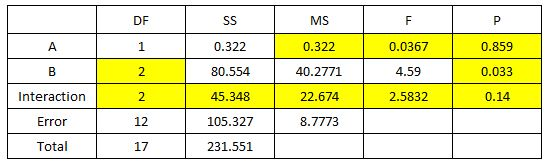
\includegraphics[width=140mm, height=26mm]{fig2.jpg}
\vspace{2 mm}

(b) 3 \\
(c) 3 \\
(d) From the p-values, it's found that only B is significant. \\

\section{ Exercise 5.3}
\textit{(a) Analyze the data and draw conclusions. Use  $\alpha = 0.05$} \\
\begin{knitrout}
\definecolor{shadecolor}{rgb}{0.969, 0.969, 0.969}\color{fgcolor}\begin{kframe}
\begin{alltt}
\hlfunctioncall{setwd}(\hlstring{"C:/Users/Subasish/Dropbox/A Spring 2014/Dr Novelo/HW"})
yield <- \hlfunctioncall{read.csv}(\hlstring{"5.3.csv"})
yield$Pressure <- \hlfunctioncall{as.factor}(yield$Pressure)
yield$Temperature <- \hlfunctioncall{as.factor}(yield$Temperature)
yield.aov <- \hlfunctioncall{aov}(Yield ~ Pressure * Temperature, data = yield)
\hlfunctioncall{summary}(yield.aov)
\end{alltt}
\begin{verbatim}
##                      Df Sum Sq Mean Sq F value  Pr(>F)    
## Pressure              2  0.768   0.384   21.59 0.00037 ***
## Temperature           2  0.301   0.151    8.47 0.00854 ** 
## Pressure:Temperature  4  0.069   0.017    0.97 0.47001    
## Residuals             9  0.160   0.018                    
## ---
## Signif. codes:  0 '***' 0.001 '**' 0.01 '*' 0.05 '.' 0.1 ' ' 1
\end{verbatim}
\end{kframe}
\end{knitrout}

From the R code values, the F-value for pressure is 21.594 with a corresponding p-value of 0.00037 and the F-value for temperature is 8.469 with a corresponding p-value of 0.0085. From these values, we understand that both pressure and temperature are significant. The interaction of pressure and temperature is not significant (because of its higher p-value.) \\

\vspace{2 mm}
\textit{(b) Prepare appropriate residual plots and comment on the model's adequacy.}\\
\begin{knitrout}
\definecolor{shadecolor}{rgb}{0.969, 0.969, 0.969}\color{fgcolor}\begin{kframe}
\begin{alltt}
\hlfunctioncall{par}(mfrow = \hlfunctioncall{c}(2, 2))
\hlfunctioncall{plot}(yield.aov)
\end{alltt}
\end{kframe}
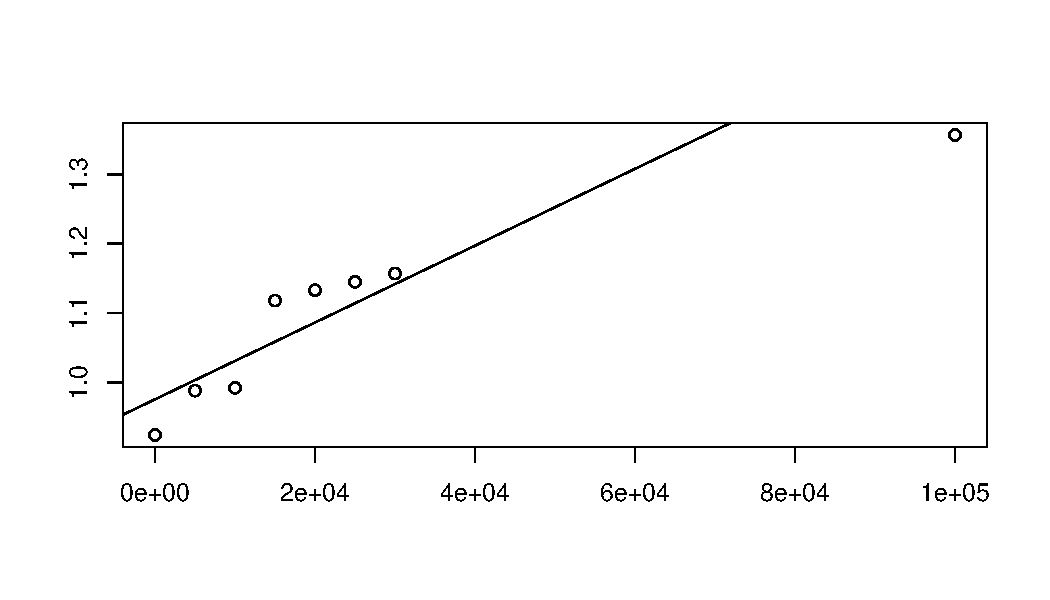
\includegraphics[width=\maxwidth]{figure/unnamed-chunk-3} 

\end{knitrout}


\begin{knitrout}
\definecolor{shadecolor}{rgb}{0.969, 0.969, 0.969}\color{fgcolor}\begin{kframe}
\begin{alltt}
\hlfunctioncall{par}(mfrow = \hlfunctioncall{c}(1, 2))
\hlfunctioncall{stripchart}(\hlfunctioncall{residuals}(yield.aov) ~ yield$Temperature, vertical = TRUE, jitter = 0, 
    xlab = \hlstring{"Temperature"}, ylab = \hlstring{"Residuals"}, cex = 1, pch = 20, main = \hlstring{"Residuals vs. Temperature"})
\hlfunctioncall{abline}(h = 0, col = \hlstring{"black"}, lty = 3)
\hlfunctioncall{stripchart}(\hlfunctioncall{residuals}(yield.aov) ~ yield$Pressure, vertical = TRUE, jitter = 0, 
    xlab = \hlstring{"Pressure"}, ylab = \hlstring{"Residuals"}, cex = 1, pch = 20, main = \hlstring{"Residuals vs. Pressure"})
\hlfunctioncall{abline}(h = 0, col = \hlstring{"black"}, lty = 3)
\end{alltt}
\end{kframe}
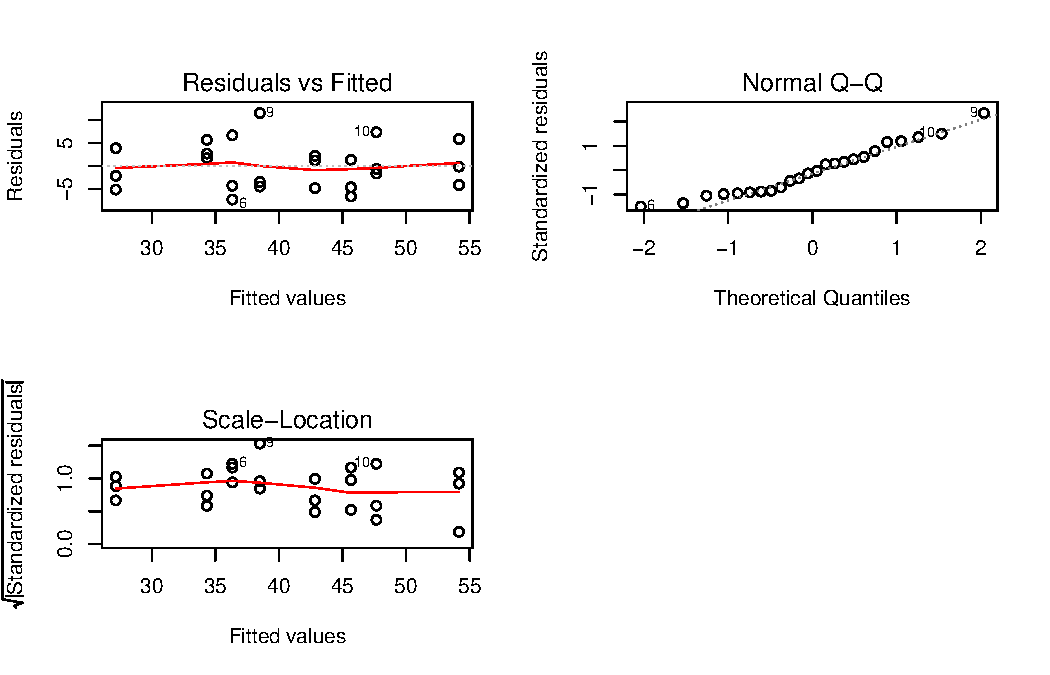
\includegraphics[width=\maxwidth]{figure/unnamed-chunk-4} 

\end{knitrout}

By observing the residual plots, no significant deviations from the observations are noticed. \\
\vspace{2 mm}

\textit{(c) Under what conditions would you operate this process?}\\
\begin{knitrout}
\definecolor{shadecolor}{rgb}{0.969, 0.969, 0.969}\color{fgcolor}\begin{kframe}
\begin{alltt}
\hlfunctioncall{library}(ggplot2)
df <- \hlfunctioncall{with}(yield, \hlfunctioncall{aggregate}(Yield, \hlfunctioncall{list}(Temperature = Temperature, Pressure = Pressure), 
    mean))
df$se <- \hlfunctioncall{with}(yield, \hlfunctioncall{aggregate}(Yield, \hlfunctioncall{list}(Temperature = Temperature, Pressure = Pressure), 
    \hlfunctioncall{function}(x) \hlfunctioncall{sd}(x)/\hlfunctioncall{sqrt}(10)))[, 3]

opar <- \hlfunctioncall{theme_update}(panel.grid.major = \hlfunctioncall{element_blank}(), panel.grid.minor = \hlfunctioncall{element_blank}(), 
    panel.background = \hlfunctioncall{element_rect}(colour = \hlstring{"black"}))
gp <- \hlfunctioncall{ggplot}(df, \hlfunctioncall{aes}(x = Pressure, y = x, colour = Temperature, group = Temperature))
gp + \hlfunctioncall{geom_line}(\hlfunctioncall{aes}(linetype = Temperature), size = 0.6) + \hlfunctioncall{geom_point}(\hlfunctioncall{aes}(shape = Temperature), 
    size = 3) + \hlfunctioncall{geom_errorbar}(\hlfunctioncall{aes}(ymax = x + se, ymin = x - se), width = 0.1)
\end{alltt}
\end{kframe}
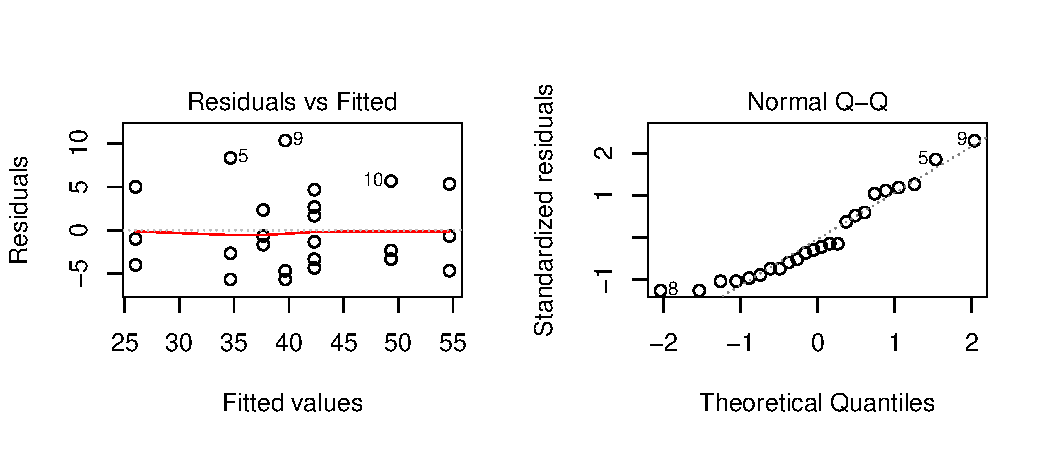
\includegraphics[width=\maxwidth]{figure/unnamed-chunk-51} 
\begin{kframe}\begin{alltt}
\hlfunctioncall{theme_set}(opar)

\hlcomment{#### Response Surface Plot}
\hlfunctioncall{library}(lattice)
\hlfunctioncall{wireframe}(Yield ~ Pressure * Temperature, data = yield, screen = \hlfunctioncall{list}(z = -45, 
    x = -45), colorkey = FALSE, shade = TRUE, light.source = \hlfunctioncall{c}(0, 10, 10), zlim = \hlfunctioncall{range}(\hlfunctioncall{seq}(90, 
    91, by = 0.05)))
\end{alltt}
\end{kframe}
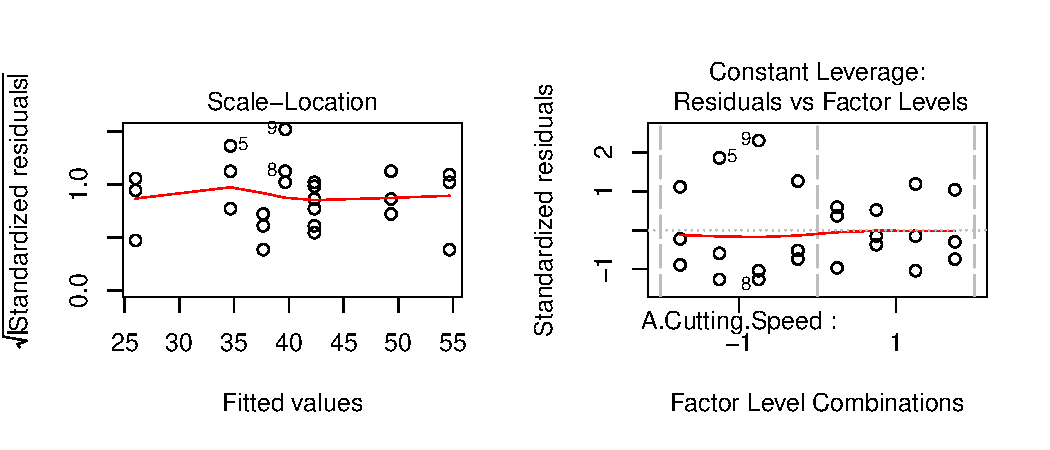
\includegraphics[width=\maxwidth]{figure/unnamed-chunk-52} 

\end{knitrout}

From the interaction plot, it's visible that temperature at 170 and pressure at 215 gives the highest yield.

\vspace{3 mm}

\section{ Exercise 5.12}
\begin{knitrout}
\definecolor{shadecolor}{rgb}{0.969, 0.969, 0.969}\color{fgcolor}\begin{kframe}
\begin{alltt}
\hlfunctioncall{TukeyHSD}(yield.aov, which = \hlstring{"Pressure"}, conf.level = 0.95)
\end{alltt}
\begin{verbatim}
##   Tukey multiple comparisons of means
##     95% family-wise confidence level
## 
## Fit: aov(formula = Yield ~ Pressure * Temperature, data = yield)
## 
## $Pressure
##            diff     lwr     upr  p adj
## 215-200  0.3167  0.1017  0.5316 0.0067
## 230-200 -0.1833 -0.3983  0.0316 0.0945
## 230-215 -0.5000 -0.7149 -0.2851 0.0003
\end{verbatim}
\begin{alltt}
\hlfunctioncall{par}(mfrow = \hlfunctioncall{c}(1, 3))
\hlfunctioncall{plot}(\hlfunctioncall{TukeyHSD}(yield.aov), cex = 0.8)
\end{alltt}
\end{kframe}
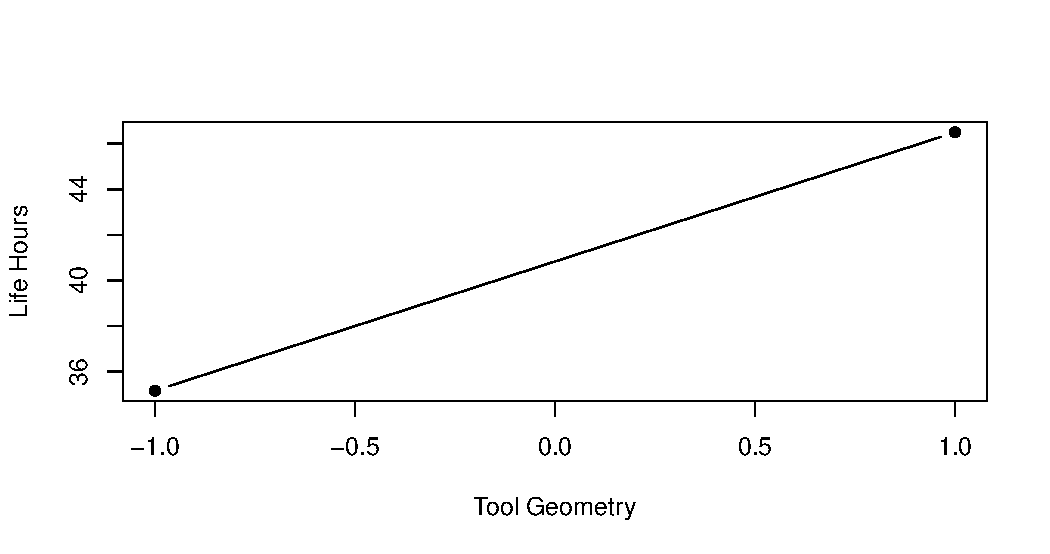
\includegraphics[width=\maxwidth]{figure/unnamed-chunk-6} 

\end{knitrout}


Three different ranges of pressure are compared. Pressure range of 230 to 200 is insignificant because of its higher p-value (greater than 0.05). The difference in pressure range (230-215) seems more than the other two pressure range. \\

\vspace{2 mm}

\section{ Exercise 5.15}

\begin{knitrout}
\definecolor{shadecolor}{rgb}{0.969, 0.969, 0.969}\color{fgcolor}\begin{kframe}
\begin{alltt}
\hlfunctioncall{setwd}(\hlstring{"C:/Users/Subasish/Dropbox/A Spring 2014/Dr Novelo/HW"})
exp <- \hlfunctioncall{read.csv}(\hlstring{"5.15.csv"})
exp$Row <- \hlfunctioncall{as.factor}(exp$Row)
exp$Column <- \hlfunctioncall{as.factor}(exp$Column)
exp.aov <- \hlfunctioncall{aov}(Data ~ Row * Column, data = exp)
\hlfunctioncall{anova}(exp.aov)
\end{alltt}


{\ttfamily\noindent\color{warningcolor}{\#\# Warning: ANOVA F-tests on an essentially perfect fit are unreliable}}\begin{verbatim}
## Analysis of Variance Table
## 
## Response: Data
##            Df Sum Sq Mean Sq F value Pr(>F)
## Row         2    581   290.3               
## Column      3     29     9.6               
## Row:Column  6     29     4.8               
## Residuals   0      0
\end{verbatim}
\begin{alltt}

\hlcomment{## As F-values can't be determined in this test, we condider anova without}
\hlcomment{## any interaction.}
exp.aov_noint <- \hlfunctioncall{aov}(Data ~ Row + Column, data = exp)
\hlfunctioncall{anova}(exp.aov_noint)
\end{alltt}
\begin{verbatim}
## Analysis of Variance Table
## 
## Response: Data
##           Df Sum Sq Mean Sq F value  Pr(>F)    
## Row        2    581   290.3   60.40 0.00011 ***
## Column     3     29     9.6    2.01 0.21472    
## Residuals  6     29     4.8                    
## ---
## Signif. codes:  0 '***' 0.001 '**' 0.01 '*' 0.05 '.' 0.1 ' ' 1
\end{verbatim}
\end{kframe}
\end{knitrout}

\vspace{2 mm}
By considering interaction, the F-value and p-values are not generated. When we consider there's no interaction, the p-values for row is very low (less than 0.05) which indicates significance.\\
\begin{knitrout}
\definecolor{shadecolor}{rgb}{0.969, 0.969, 0.969}\color{fgcolor}\begin{kframe}
\begin{alltt}
\hlfunctioncall{library}(asbio)
\end{alltt}


{\ttfamily\noindent\color{warningcolor}{\#\# Warning: package 'asbio' was built under R version 3.0.3}}

{\ttfamily\noindent\itshape\color{messagecolor}{\#\# Loading required package: tcltk}}\begin{alltt}
\hlfunctioncall{setwd}(\hlstring{"C:/Users/Subasish/Dropbox/A Spring 2014/Dr Novelo/HW"})
exp <- \hlfunctioncall{read.csv}(\hlstring{"5.15.csv"})
\hlfunctioncall{tukey.add.test}(exp$Data, exp$Row, exp$Column)
\end{alltt}
\begin{verbatim}
## 
## Tukey's one df test for additivity 
## F = 0.6999   Denom df = 5    p-value = 0.441
\end{verbatim}
\begin{alltt}
\hlcomment{### From the test}
F_nonadd = 0.6999
df_nonadd = 1
ss_nonadd = 3.54
ms_nonadd = ss_nonadd/df_nonadd
ss_err = 28.83 - ss_nonadd
df_err = 6 - df_nonadd
ms_err = ss_err/df_err
F_row = 580.5
F_col = 28.92
df_row = 2
df_col = 3
p_nonadd = 1 - \hlfunctioncall{pf}(F_nonadd, df_nonadd, df_err)
p_row = 1 - \hlfunctioncall{pf}(F_row, df_col, df_err)
p_col = 1 - \hlfunctioncall{pf}(F_col, df_col, df_err)
\hlfunctioncall{rbind}(p_row, p_col, p_nonadd)
\end{alltt}
\begin{verbatim}
##               [,1]
## p_row    8.925e-07
## p_col    1.384e-03
## p_nonadd 4.410e-01
\end{verbatim}
\end{kframe}
\end{knitrout}


\vspace{2 mm}
\raggedright{The ANOVA Table (including Nonadditivity row):}\\
\vspace{2 mm}
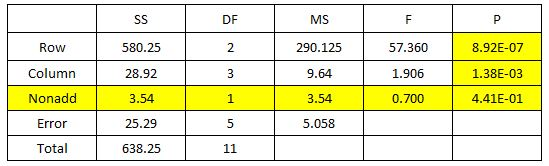
\includegraphics[width=140mm, height=28mm]{fig5a.jpg}\\

\vspace{2 mm}
From Tukey's one df test for additivity, the p-value is high enough (greater than 0.05). So, we can't reject the null hypothesis. \\

\section{ Exercise 5.21}
\begin{knitrout}
\definecolor{shadecolor}{rgb}{0.969, 0.969, 0.969}\color{fgcolor}\begin{kframe}
\begin{alltt}
\hlfunctioncall{setwd}(\hlstring{"C:/Users/Subasish/Dropbox/A Spring 2014/Dr Novelo/HW"})
yield2 <- \hlfunctioncall{read.csv}(\hlstring{"5.21a.csv"})
\hlfunctioncall{head}(yield2, n = 2)
\end{alltt}
\begin{verbatim}
##   Pressure Temperature Day Yield
## 1      250         Low   1  86.3
## 2      250         Low   2  86.1
\end{verbatim}
\begin{alltt}
\hlfunctioncall{library}(easyanova)  \hlcomment{## \hlstring{'easyanova'} package is utilized for convenience.}
\end{alltt}


{\ttfamily\noindent\itshape\color{messagecolor}{\#\# Loading required package: car}}

{\ttfamily\noindent\itshape\color{messagecolor}{\#\# Loading required package: MASS}}

{\ttfamily\noindent\itshape\color{messagecolor}{\#\# Loading required package: nnet}}

{\ttfamily\noindent\itshape\color{messagecolor}{\#\# Loading required package: nlme}}\begin{alltt}
r1 = \hlfunctioncall{ea2}(yield2, design = 2)
\end{alltt}
\end{kframe}
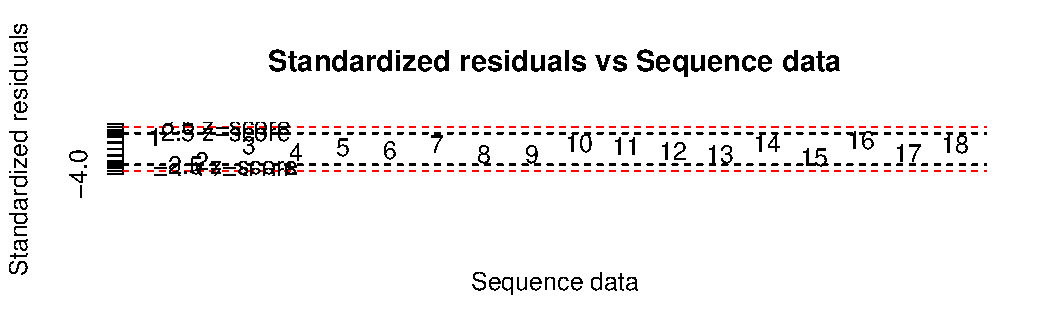
\includegraphics[width=\maxwidth]{figure/unnamed-chunk-9} 
\begin{kframe}\begin{alltt}
r1[[1]]
\end{alltt}
\begin{verbatim}
##                   df type III SS mean square F value    p>F
## factor_1           2       5.508      2.7539  5.1838  0.036
## factor_2           2      99.854     49.9272 93.9807 <0.001
## blocks             1      13.005     13.0050   24.48 0.0011
## factor_1:factor_2  4       4.452      1.1131  2.0952 0.1733
## Residuals          8       4.250      0.5312       -      -
\end{verbatim}
\end{kframe}
\end{knitrout}

From the ANOVA table values, it is easily interpreted that both temperature and pressure have significant effects. The usage of blocks is also significant. The interaction of temperature and pressure is not significant (greater than 0.05) in this experiment.\\
\vspace{2 mm}

\section{ Exercise 5.24}

\textit{(a) Analyze the data from this experiment. Use  $\alpha = 0.05$ }\\
\begin{knitrout}
\definecolor{shadecolor}{rgb}{0.969, 0.969, 0.969}\color{fgcolor}\begin{kframe}
\begin{alltt}
\hlfunctioncall{setwd}(\hlstring{"C:/Users/Subasish/Dropbox/A Spring 2014/Dr Novelo/HW"})
environ <- \hlfunctioncall{read.csv}(\hlstring{"5.24.csv"})
environ$Frequency <- \hlfunctioncall{as.factor}(environ$Frequency)
environ.aov <- \hlfunctioncall{aov}(Crack.Growth ~ Frequency * Environment, data = environ)
\hlfunctioncall{summary}(environ.aov)
\end{alltt}
\begin{verbatim}
##                       Df Sum Sq Mean Sq F value  Pr(>F)    
## Frequency              2  209.9   104.9     522 < 2e-16 ***
## Environment            2   64.3    32.1     160 1.1e-15 ***
## Frequency:Environment  4  102.0    25.5     127 < 2e-16 ***
## Residuals             27    5.4     0.2                    
## ---
## Signif. codes:  0 '***' 0.001 '**' 0.01 '*' 0.05 '.' 0.1 ' ' 1
\end{verbatim}
\end{kframe}
\end{knitrout}


Both frequency and environment as well as the interaction between them are significant because of their low p-values (less than 0.05).\\

\vspace{2 mm}

\textit{(b) Analyze the residuals.}\\

\begin{knitrout}
\definecolor{shadecolor}{rgb}{0.969, 0.969, 0.969}\color{fgcolor}\begin{kframe}
\begin{alltt}
\hlfunctioncall{par}(mfrow = \hlfunctioncall{c}(2, 2))
\hlfunctioncall{plot}(environ.aov)
\end{alltt}
\end{kframe}
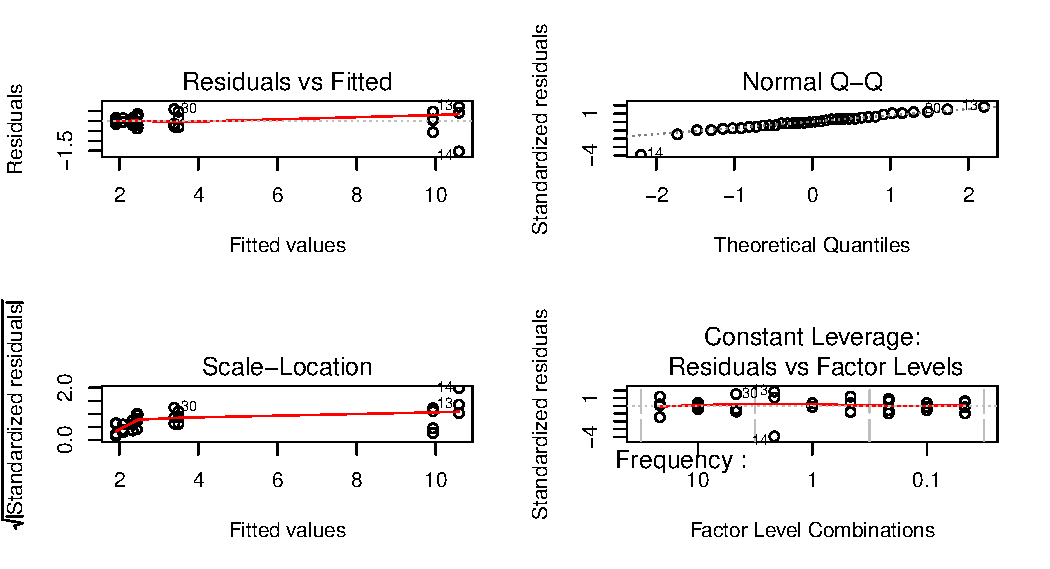
\includegraphics[width=\maxwidth]{figure/unnamed-chunk-11} 

\end{knitrout}


\begin{knitrout}
\definecolor{shadecolor}{rgb}{0.969, 0.969, 0.969}\color{fgcolor}\begin{kframe}
\begin{alltt}
\hlfunctioncall{par}(mfrow = \hlfunctioncall{c}(1, 2))
\hlfunctioncall{stripchart}(\hlfunctioncall{residuals}(environ.aov) ~ environ$Environment, vertical = TRUE, jitter = 0, 
    xlab = \hlstring{"Environment"}, ylab = \hlstring{"Residuals"}, cex = 1.1, pch = 20, main = \hlstring{"Residuals vs. Environment"})
\hlfunctioncall{abline}(h = 0, col = \hlstring{"black"}, lty = 3)
\hlfunctioncall{stripchart}(\hlfunctioncall{residuals}(environ.aov) ~ environ$Frequency, vertical = TRUE, jitter = 0, 
    xlab = \hlstring{"Frequency"}, ylab = \hlstring{"Residuals"}, cex = 1.1, pch = 20, main = \hlstring{"Residuals vs. Frequency"})
\hlfunctioncall{abline}(h = 0, col = \hlstring{"black"}, lty = 3)
\end{alltt}
\end{kframe}
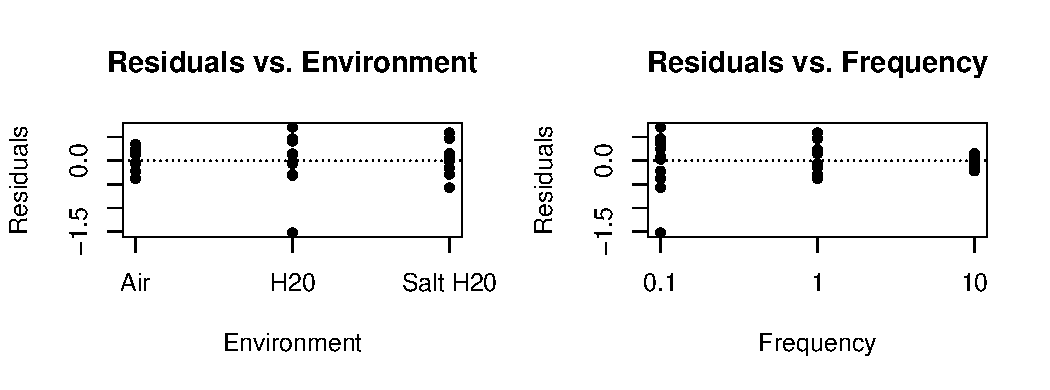
\includegraphics[width=\maxwidth]{figure/unnamed-chunk-12} 

\end{knitrout}


The inequality of variance seems problematic from the observation of the residuals plots. This is visible on the plots of residuals versus predicted response and the plots of residuals versus frequency.\\

\vspace{2 mm}

\textit{(c) Repeat the analyses from parts (a) and (b) using ln(y) as the response. Comment on the results.}\\

\begin{knitrout}
\definecolor{shadecolor}{rgb}{0.969, 0.969, 0.969}\color{fgcolor}\begin{kframe}
\begin{alltt}
environ1.aov <- \hlfunctioncall{aov}(\hlfunctioncall{log}(Crack.Growth) ~ Frequency * Environment, data = environ)
\hlfunctioncall{summary}(environ1.aov)
\end{alltt}
\begin{verbatim}
##                       Df Sum Sq Mean Sq F value  Pr(>F)    
## Frequency              2   7.57    3.79   404.1 < 2e-16 ***
## Environment            2   2.36    1.18   125.8 2.1e-14 ***
## Frequency:Environment  4   3.53    0.88    94.2 1.9e-15 ***
## Residuals             27   0.25    0.01                    
## ---
## Signif. codes:  0 '***' 0.001 '**' 0.01 '*' 0.05 '.' 0.1 ' ' 1
\end{verbatim}
\begin{alltt}
\hlfunctioncall{par}(mfrow = \hlfunctioncall{c}(2, 2))
\hlfunctioncall{plot}(environ1.aov)
\end{alltt}
\end{kframe}
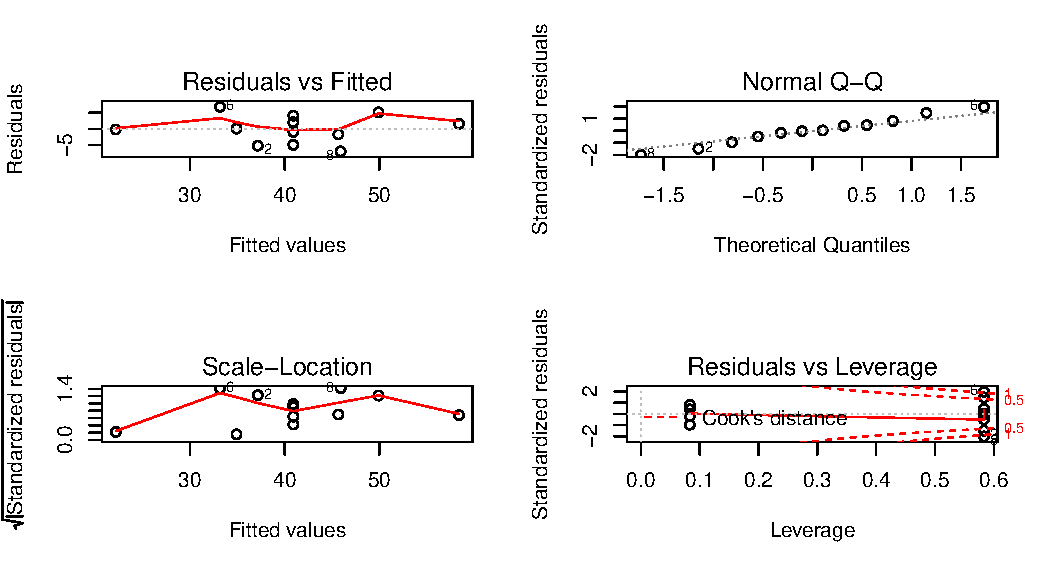
\includegraphics[width=\maxwidth]{figure/unnamed-chunk-13} 

\end{knitrout}


\begin{knitrout}
\definecolor{shadecolor}{rgb}{0.969, 0.969, 0.969}\color{fgcolor}\begin{kframe}
\begin{alltt}
\hlfunctioncall{par}(mfrow = \hlfunctioncall{c}(1, 2))
\hlfunctioncall{stripchart}(\hlfunctioncall{residuals}(environ1.aov) ~ environ$Environment, vertical = TRUE, jitter = 0, 
    xlab = \hlstring{"Environment"}, ylab = \hlstring{"Residuals"}, cex = 1.1, pch = 20, main = \hlstring{"Residuals vs. Environment"})
\hlfunctioncall{abline}(h = 0, col = \hlstring{"black"}, lty = 3)
\hlfunctioncall{abline}(h = 0, col = \hlstring{"black"}, lty = 3)
\hlfunctioncall{stripchart}(\hlfunctioncall{residuals}(environ1.aov) ~ environ$Frequency, vertical = TRUE, jitter = 0, 
    xlab = \hlstring{"Frequency"}, ylab = \hlstring{"Residuals"}, cex = 1.1, pch = 20, main = \hlstring{"Residuals vs. Frequency"})
\hlfunctioncall{abline}(h = 0, col = \hlstring{"black"}, lty = 3)
\hlfunctioncall{abline}(h = 0, col = \hlstring{"black"}, lty = 3)
\end{alltt}
\end{kframe}
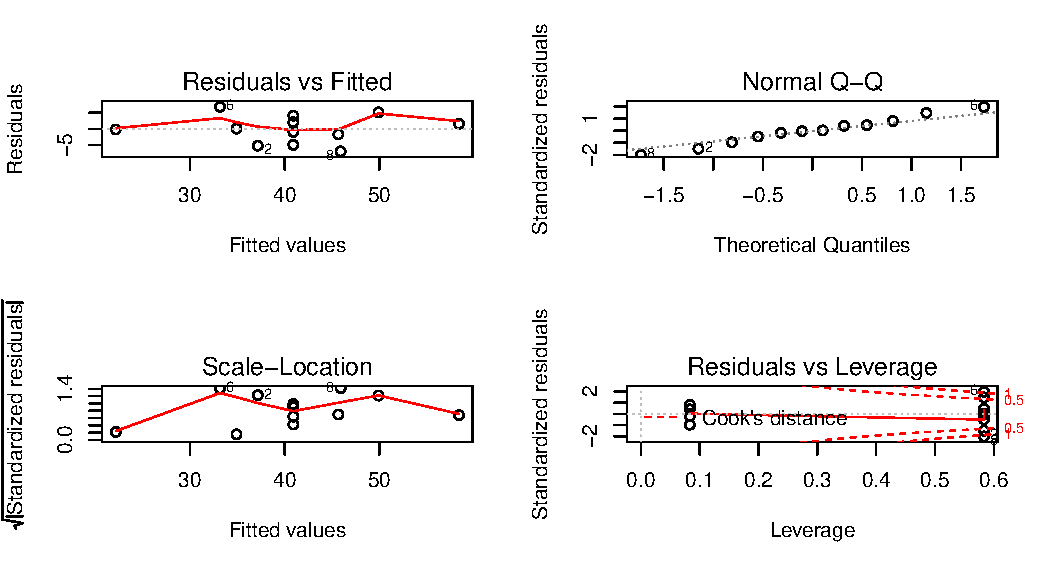
\includegraphics[width=\maxwidth]{figure/unnamed-chunk-14} 

\end{knitrout}


From the transformed data, both frequency and environment as well as their interaction are significant. The residual plots on the transformed data seems better than the original data. \\

\vspace{2 mm}

\section{ Exercise 5.26}

\textit{(a) Analyze the data and draw conclusions. Use  $\alpha = 0.05$} \\
\begin{knitrout}
\definecolor{shadecolor}{rgb}{0.969, 0.969, 0.969}\color{fgcolor}\begin{kframe}
\begin{alltt}
\hlfunctioncall{setwd}(\hlstring{"C:/Users/Subasish/Dropbox/A Spring 2014/Dr Novelo/HW"})
battaries <- \hlfunctioncall{read.csv}(\hlstring{"5.26.csv"})
battaries.aov <- \hlfunctioncall{aov}(Life.Hours ~ Battery * Device, data = battaries)
\hlfunctioncall{summary}(battaries.aov)
\end{alltt}
\begin{verbatim}
##                Df Sum Sq Mean Sq F value  Pr(>F)    
## Battery         1   0.80    0.80    9.33   0.022 *  
## Device          2  22.45   11.22  130.75 1.1e-05 ***
## Battery:Device  2   0.08    0.04    0.48   0.643    
## Residuals       6   0.52    0.09                    
## ---
## Signif. codes:  0 '***' 0.001 '**' 0.01 '*' 0.05 '.' 0.1 ' ' 1
\end{verbatim}
\end{kframe}
\end{knitrout}


From the p-values, we can say that both the battery and device are significant (p-values are less than 0.05), but the interaction between them is not significant (p value is greater than 0.05).\\

\vspace{2 mm}

\textit{(b) Investigate model adequacy by plotting the residuals.}\\
\begin{knitrout}
\definecolor{shadecolor}{rgb}{0.969, 0.969, 0.969}\color{fgcolor}\begin{kframe}
\begin{alltt}
\hlfunctioncall{par}(mfrow = \hlfunctioncall{c}(2, 2))
\hlfunctioncall{plot}(battaries.aov)
\end{alltt}
\end{kframe}
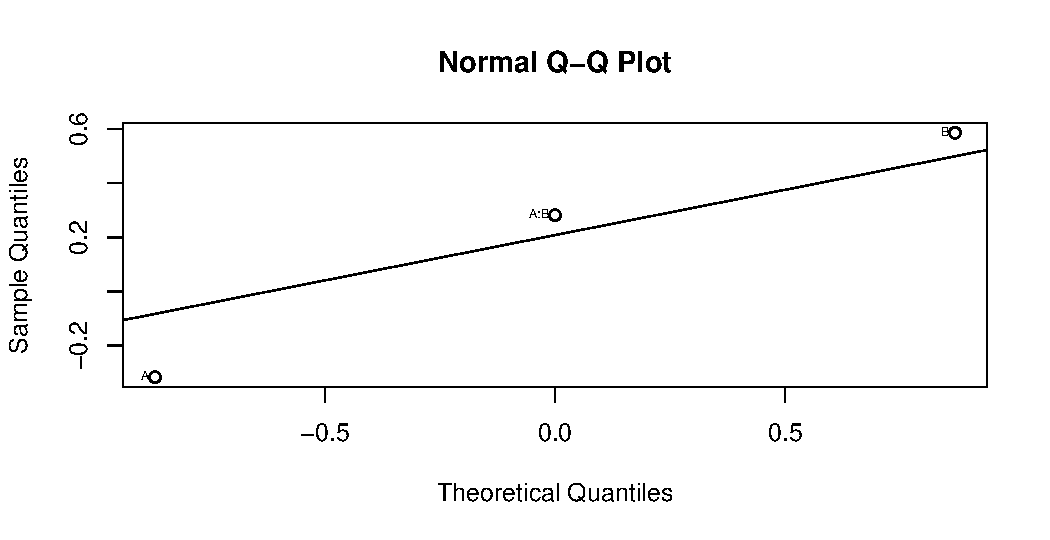
\includegraphics[width=\maxwidth]{figure/unnamed-chunk-16} 

\end{knitrout}


\begin{knitrout}
\definecolor{shadecolor}{rgb}{0.969, 0.969, 0.969}\color{fgcolor}\begin{kframe}
\begin{alltt}
\hlfunctioncall{par}(mfrow = \hlfunctioncall{c}(1, 2))
\hlfunctioncall{stripchart}(\hlfunctioncall{residuals}(battaries.aov) ~ battaries$Battery, method = \hlstring{"stack"}, vertical = TRUE, 
    jitter = 0, xlab = \hlstring{"Battaries"}, ylab = \hlstring{"Residuals"}, cex = 1.1, pch = 20, 
    main = \hlstring{"Residuals vs. Battaries"})

\hlfunctioncall{stripchart}(\hlfunctioncall{residuals}(battaries.aov) ~ battaries$Device, method = \hlstring{"stack"}, vertical = TRUE, 
    jitter = 0, xlab = \hlstring{"Device"}, ylab = \hlstring{"Residuals"}, cex = 1.1, pch = 20, main = \hlstring{"Residuals vs. Device"})
\end{alltt}
\end{kframe}
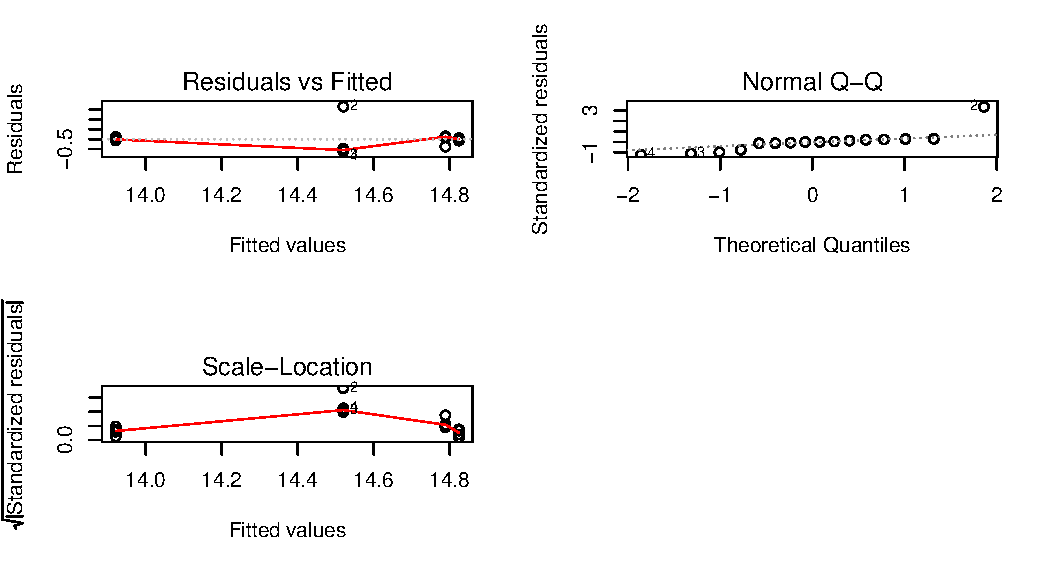
\includegraphics[width=\maxwidth]{figure/unnamed-chunk-17} 

\end{knitrout}


By observing the residual plots, no significant variation from the assumption is visible. \\

\vspace{2 mm}

\textit{(c) Which brand of batteries would you recommend?}\\

\begin{knitrout}
\definecolor{shadecolor}{rgb}{0.969, 0.969, 0.969}\color{fgcolor}\begin{kframe}
\begin{alltt}
df <- \hlfunctioncall{with}(battaries, \hlfunctioncall{aggregate}(Life.Hours, \hlfunctioncall{list}(Device = Device, Battery = Battery), 
    mean))
df$se <- \hlfunctioncall{with}(battaries, \hlfunctioncall{aggregate}(Life.Hours, \hlfunctioncall{list}(Device = Device, Battery = Battery), 
    \hlfunctioncall{function}(x) \hlfunctioncall{sd}(x)/\hlfunctioncall{sqrt}(10)))[, 3]

opar <- \hlfunctioncall{theme_update}(panel.grid.major = \hlfunctioncall{element_blank}(), panel.grid.minor = \hlfunctioncall{element_blank}(), 
    panel.background = \hlfunctioncall{element_rect}(colour = \hlstring{"black"}))
gp <- \hlfunctioncall{ggplot}(df, \hlfunctioncall{aes}(x = Battery, y = x, colour = Device, group = Device))
gp + \hlfunctioncall{geom_line}(\hlfunctioncall{aes}(linetype = Device), size = 0.6) + \hlfunctioncall{geom_point}(\hlfunctioncall{aes}(shape = Device), 
    size = 3) + \hlfunctioncall{geom_errorbar}(\hlfunctioncall{aes}(ymax = x + se, ymin = x - se), width = 0.1)
\end{alltt}
\end{kframe}
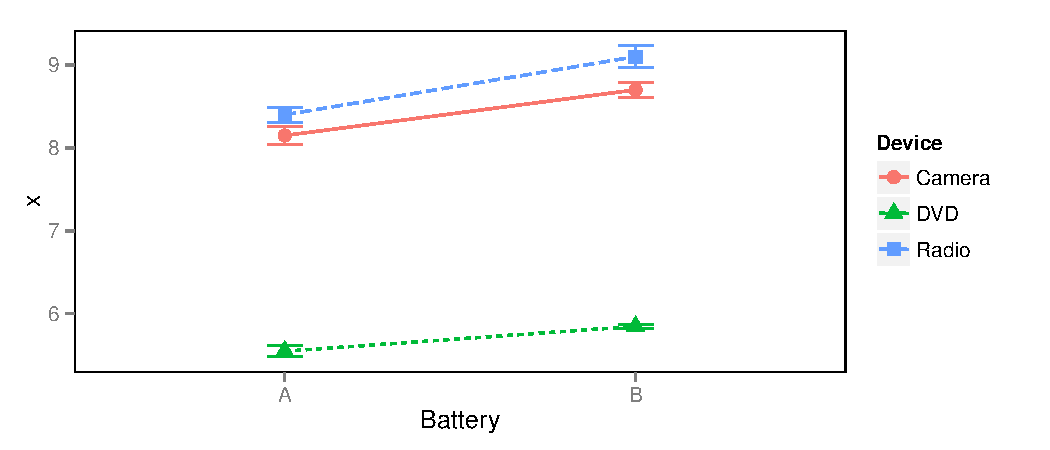
\includegraphics[width=\maxwidth]{figure/unnamed-chunk-18} 

\end{knitrout}


From the interaction, we can recommend battery brand B. \\

\vspace{2 mm}


\section{ Exercise 5.43}
\begin{knitrout}
\definecolor{shadecolor}{rgb}{0.969, 0.969, 0.969}\color{fgcolor}\begin{kframe}
\begin{alltt}
\hlcomment{## Given}
ss_tot = 1000
ss_err = 150
ss_a = 350
ss_b = 300
ss_ab = 200
df_a = 2
df_err = 18
ms_b = 150
ms_ab = 50

ms_a = ss_a/df_a
df_b = ss_b/ms_b
df_ab = ss_ab/ms_ab
df_tot = df_a + df_b + df_ab + df_err
ms_err = ss_err/df_err
F_a = ms_a/ms_err
F_b = ms_b/ms_err
F_ab = ms_ab/ms_err
p_a = 1 - \hlfunctioncall{pf}(F_a, df_a, df_err)
p_b = 1 - \hlfunctioncall{pf}(F_b, df_b, df_err)
p_ab = 1 - \hlfunctioncall{pf}(F_ab, df_ab, df_err)

\hlfunctioncall{rbind}(df_b, df_ab, df_tot)
\end{alltt}
\begin{verbatim}
##        [,1]
## df_b      2
## df_ab     4
## df_tot   26
\end{verbatim}
\begin{alltt}
\hlfunctioncall{rbind}(ms_a, ms_err)
\end{alltt}
\begin{verbatim}
##           [,1]
## ms_a   175.000
## ms_err   8.333
\end{verbatim}
\begin{alltt}
\hlfunctioncall{rbind}(F_a, F_b, F_ab)
\end{alltt}
\begin{verbatim}
##      [,1]
## F_a    21
## F_b    18
## F_ab    6
\end{verbatim}
\begin{alltt}
\hlfunctioncall{rbind}(p_a, p_b, p_ab)
\end{alltt}
\begin{verbatim}
##           [,1]
## p_a  1.968e-05
## p_b  5.081e-05
## p_ab 2.996e-03
\end{verbatim}
\begin{alltt}

\hlcomment{## standard deviation of response variable}
sd = \hlfunctioncall{sqrt}(ms_err)
sd
\end{alltt}
\begin{verbatim}
## [1] 2.887
\end{verbatim}
\end{kframe}
\end{knitrout}


\vspace{2 mm}
\raggedright{The ANOVA Table:}\\
\vspace{2 mm}
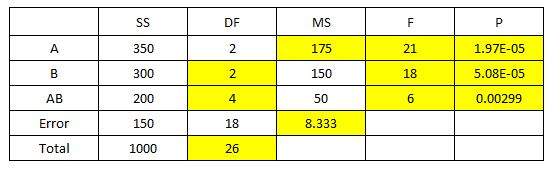
\includegraphics[width=140mm, height=30mm]{fig3.jpg}
\vspace{2 mm}

(a) 3 \\
(b) 4 \\
(c) 8.333 \\
(d) 175 \\
(e) 3 \\
(f) The p-values for A, B and the interaction are very low (less than 0.05). So, the effect of A, B and interaction are significant. \\
(g) 2.886\\
(h) 2\\



\section{ Exercise 5.44}
\begin{knitrout}
\definecolor{shadecolor}{rgb}{0.969, 0.969, 0.969}\color{fgcolor}\begin{kframe}
\begin{alltt}
\hlcomment{## Given}
ss_tot = 1000
ss_block = 60
ss_a = 350
ss_b = 300
ss_ab = 200
n = 3

ss_err = ss_tot - ss_block - ss_a - ss_b - ss_ab
df_block = n - 1
ms_block = ss_block/df_block

\hlcomment{## From 5.43}
df_a = 2
ms_a = 175
df_b = 2
ms_b = 150
df_ab = 4
ms_ab = 50
df_tot = 26

df_err = df_tot - df_a - df_b - df_ab - df_block
ms_err = ss_err/df_err
F_a = ms_a/ms_err
F_b = ms_b/ms_err
F_ab = ms_ab/ms_err
F_block = ms_block/ms_err
p_a = 1 - \hlfunctioncall{pf}(F_a, df_a, df_err)
p_b = 1 - \hlfunctioncall{pf}(F_b, df_b, df_err)
p_block = 1 - \hlfunctioncall{pf}(F_block, df_block, df_err)

ss_err
\end{alltt}
\begin{verbatim}
## [1] 90
\end{verbatim}
\begin{alltt}
\hlfunctioncall{rbind}(df_block, df_err, df_tot)
\end{alltt}
\begin{verbatim}
##          [,1]
## df_block    2
## df_err     16
## df_tot     26
\end{verbatim}
\begin{alltt}
\hlfunctioncall{rbind}(ms_block, ms_err)
\end{alltt}
\begin{verbatim}
##            [,1]
## ms_block 30.000
## ms_err    5.625
\end{verbatim}
\begin{alltt}
F_block
\end{alltt}
\begin{verbatim}
## [1] 5.333
\end{verbatim}
\begin{alltt}
\hlfunctioncall{rbind}(p_block, p_a, p_b)
\end{alltt}
\begin{verbatim}
##              [,1]
## p_block 1.680e-02
## p_a     3.064e-06
## p_b     8.043e-06
\end{verbatim}
\end{kframe}
\end{knitrout}


\vspace{2 mm}
\raggedright{The ANOVA Table:}\\
\vspace{2 mm}
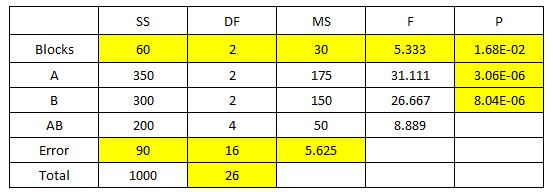
\includegraphics[width=140mm, height=32mm]{fig4.jpg}
\vspace{2 mm}

\end{document}
